
\section{Laser stand for the MAPMT characterization}
The large number of the channels in the RICH detector  poses challenging problem for the MAPMT testing and calibration.
RICH consists of 391 MAPMTs resulting in total number of channels equal to 25024. So in order to test them efficiently within a reasonable timeframe the fully automated test stand was build to evaluate 6 MAPMTs at once, as shown on Fig.~\ref{fig:MAPMTtest}.

\begin{figure}[hbt]
	\centering
	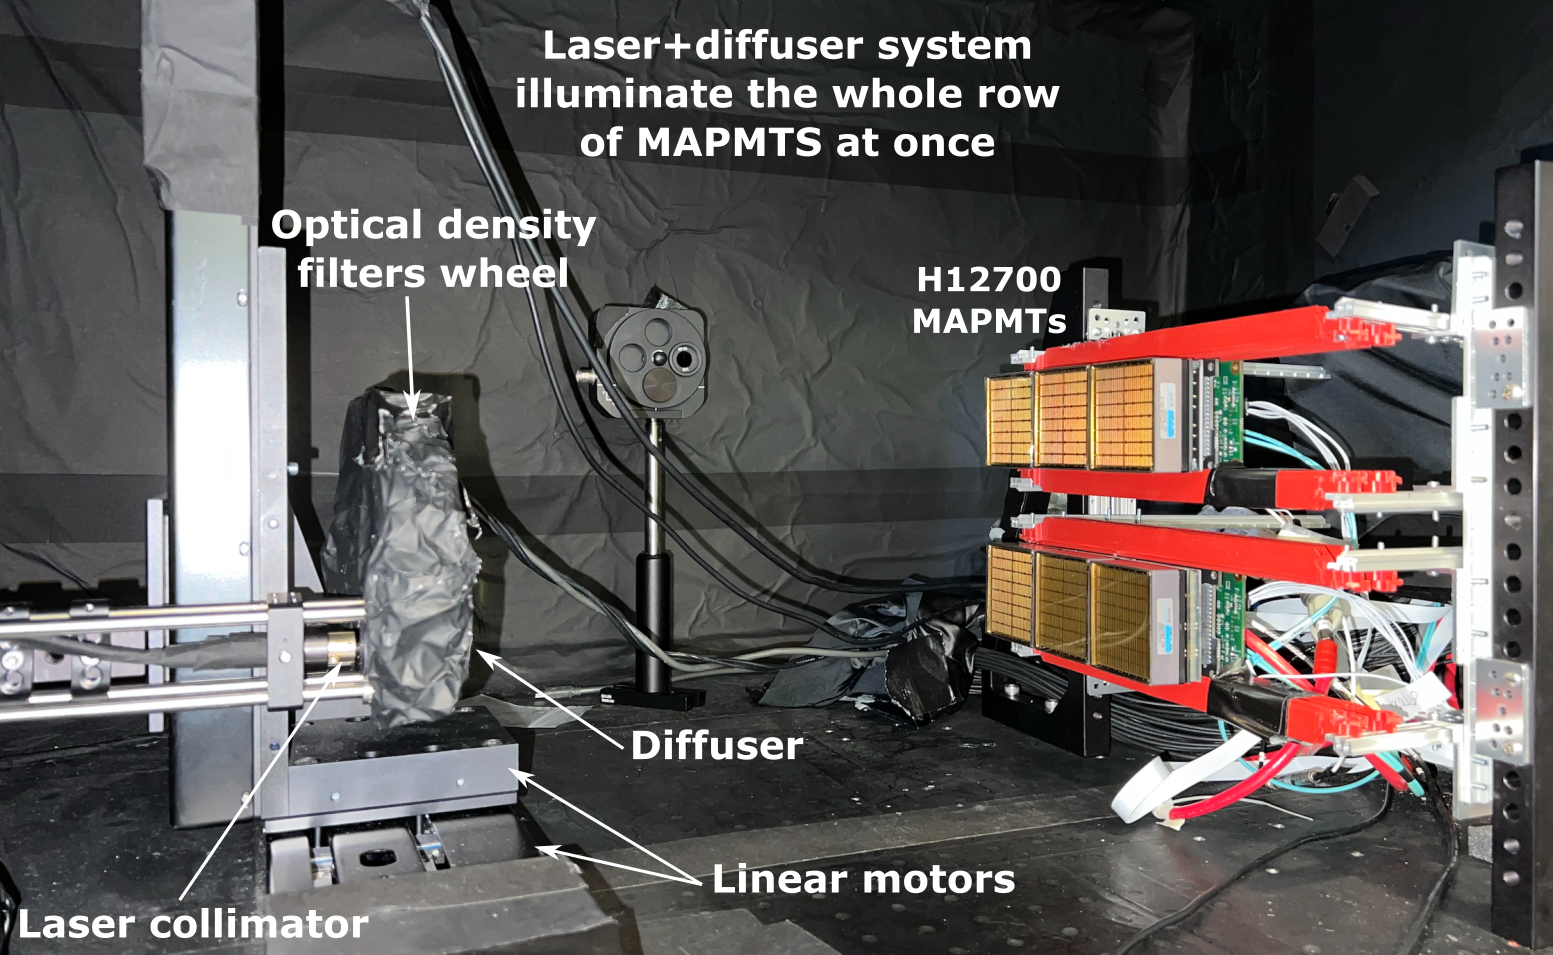
\includegraphics[width=0.9\linewidth]{figures/LaserSetup.png}
	\caption{Inner view of the laser stand.}
	\label{fig:MAPMTtest}
\end{figure}

The test stand consists of picosecond diode  laser PiL047X with 470 nm wavelength, 2 long travel motorized stands to drive laser fiber in two dimensional space for individual pixel illumination, the motorized wheel with neutral density filter system, 2 adapter boards for MAPMT with JLab designed front-end electronics boards \cite{Contalbrigo:2020}.
The laser light is directed through the fiber and attenuated to the single photon level using the neutral density filters to mimic the conditions of the RICH detector.
The motors can be remotely controlled to move the focused laser beam across (see Fig.~\ref{fig:beamopt1}) the entire surface of the MAPMT entrance window and illuminate one by one of all its 64 pixels individually.
Alternatively, the Engineered Diffuser can be used to scatter laser beam and produce square pattern with non-Gaussian intensity distribution (see Fig.~\ref{fig:beamopt2}). 
The second option is used in production mode to illuminate the full row of 3 MAPMTs at once.

All laser stand equipment is placed in the black box with non-reflective black material on the optical table. The laser interlock safety box automatically switches off laser, as well as front-end electronics low voltage and MAPMT high voltage, to prevent possible photomultiplier damage or human exposure to the laser light in case somebody attempts to open the front door of the black box during measurements.

\begin{figure}[bt]
	\centering
	\begin{subfigure}[b]{0.628\linewidth}
		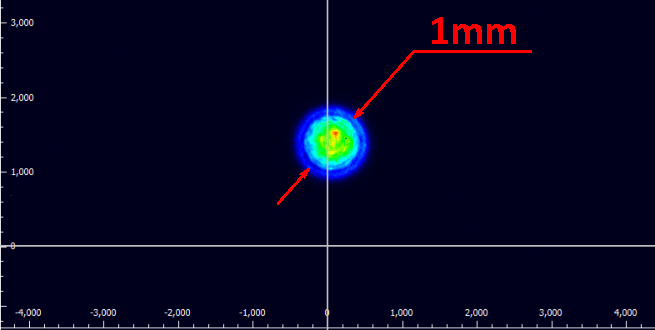
\includegraphics[width=\linewidth]{figures/beamspot.pdf}
		\caption{Focused laser beam with the dimension much less than the  MAPMT pixel size.}
		\label{fig:beamopt1}
	\end{subfigure}
	\begin{subfigure}[b]{0.354\linewidth}
		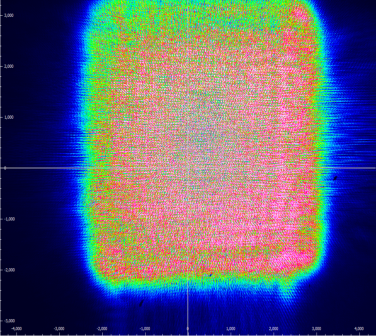
\includegraphics[width=\linewidth]{figures/beamsquare.pdf}
		\caption{Square pattern illuminated all MAPMT surface.}
		\label{fig:beamopt2}
	\end{subfigure}
	\caption{The laser light output options.}
\end{figure}

This configuration minimizes routine workload and allows the evaluation of 6 MAPMTs (equivalent to 384 conventional PMTs!) at different high voltages and different light intensities within 6 hours with less than 15 minutes of human interaction used to load the MAPMTs to the front-end boards.

